
\documentclass{article}
\usepackage[utf8]{inputenc}
\usepackage{graphicx}
\usepackage[T1]{fontenc}
\usepackage{lmodern}
\usepackage{listings}
\usepackage[numbers]{natbib} %IEEE
\usepackage{color}
\usepackage{hyperref}
\usepackage{soul}
\usepackage{float}
\usepackage{pgfplotstable}
\usepackage[font=itshape]{quoting}
\usepackage{booktabs}
\usepackage{amsmath}
\usepackage{multicol}
%\usepackage[table,xcdraw]{xcolor}

\usepackage{minted}
\usepackage[a4paper, total={6in, 8in}]{geometry}
\definecolor{dkgreen}{rgb}{0,0.6,0}
\definecolor{gray}{rgb}{0.5,0.5,0.5}
\definecolor{mauve}{rgb}{0.58,0,0.82}
\definecolor{backcolour}{rgb}{0.95,0.95,0.92}
\definecolor{codegreen}{rgb}{0,0.6,0}
% Define a custom style
\lstdefinestyle{myStyle}{
    backgroundcolor=\color{backcolour},   
    commentstyle=\color{codegreen},
    keywordstyle = \bfseries\color{mauve},
    basicstyle=\ttfamily\footnotesize,
    breakatwhitespace=false,         
    breaklines=true,                 
    keepspaces=true,                 
    numbers=left,       
    numbersep=5pt,                  
    showspaces=false,                
    showstringspaces=false,
    showtabs=false,                  
    tabsize=2,
}
\lstset{style=mystyle}

\title{Data Mining \& Machine Learning \\ \large Computer Exercise 7 - Linear Models}
\author{Steinarr Hrafn Höskuldsson}
\date{October 2022}
\newcommand{\mycomment}[1]{}

\begin{document}
\maketitle
\mycomment{
\begin{figure}[h]
    \centering
    \includegraphics[width=0.75\textwidth]{LAB3/Basic1.png}
    \caption{"Switch test" Breadboard set up}
    \label{fig:Switch_test}
\end{figure}

\lstinputlisting[caption=Defining 'ColorMatch' state, label={lst:colormatch}, language=Python, firstline=44, lastline=52]{LAB3/Basic.py}

}
\section*{Section 1.2}

\begin{figure}[H]
    \centering
    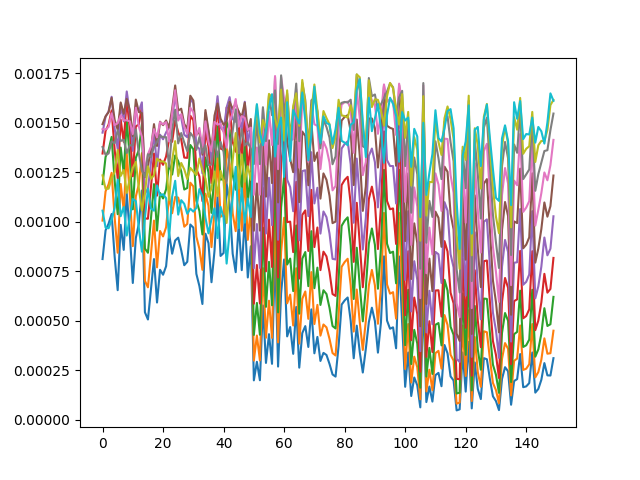
\includegraphics[width=0.75\textwidth]{07_linear_models/plot_1_2.png}
    \caption{The output of each of the basis function over the dataset}
    \label{fig:section12}
\end{figure}

\section*{Section 1.5}
\begin{figure}[H]
    \centering
    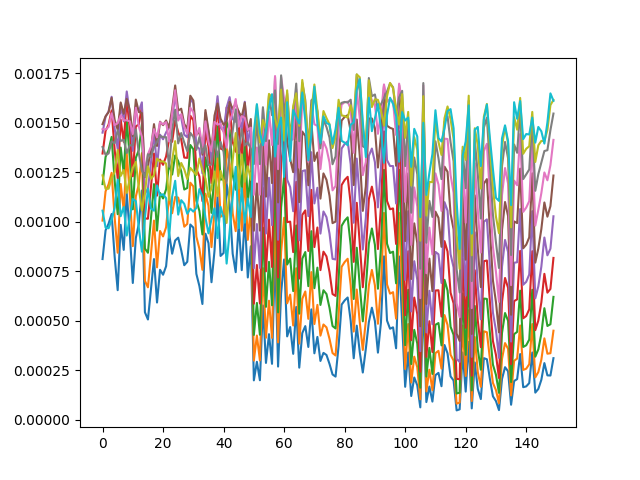
\includegraphics[width=0.75\textwidth]{07_linear_models/plot_1_2.png}
    \caption{The Actual values plotted in a scatter plot against the predicted values.}
    \label{fig:section15}
\end{figure}

Figure \ref{fig:section15} shows the Actual values plotted against the predicted values. There is practically no correlation between them. 

\section*{Independent}
A fellow student, Sigurður Ágúst Jakobsson, pointed out on Piazza that we are mixing up columns and rows when finding the min and max of each feature. By fixing that we get a slightly better scatter plot as can be seen in Figure \ref{fig:fixi}. And a little bit of trial and error with changing \verb!M! and \verb!sigma!, gives the scatter plot in Figure \ref{fig:m100s2}.

In an effort to find the optimal values for \verb!M! and \verb!sigma! a for loop was written that goes through different value combinations and saves the Mean-Square-Error of each combination.

The results were plotted in the 

\newpage
\section*{Appendix}
\appendix
\section{Code}

\lstinputlisting[ label={lst:colormatch}, language=Python, ]{07_linear_models/Steinarr7.py}


\end{document}

